\documentclass[a4paper,11pt]{article}
\usepackage[utf8]{inputenc}
\usepackage[T3,T1]{fontenc}
\usepackage[english,ngerman]{babel}
\usepackage[noenc]{tipa}
\usepackage{tipx}
\usepackage{pifont}
\usepackage{eurosym}
\usepackage{amsmath}
\usepackage{wasysym}
\usepackage{amssymb,amsfonts,textcomp}
\usepackage{color}
\usepackage{array}
\usepackage{hhline}
%\usepackage{hyperref}
\usepackage{graphicx}
\usepackage{tabularx}
%\hypersetup{pdftex, colorlinks=true, linkcolor=blue, citecolor=blue, filecolor=blue, urlcolor=blue, pdftitle=, pdfauthor=, pdfsubject=, pdfkeywords=}
\usepackage{url}
% Text styles
\newcommand\textstyleSourceText[1]{\texttt{#1}}
% Outline numbering
\setcounter{secnumdepth}{3}
\renewcommand\thesection{\arabic{section}}
% List styles
\newcommand\liststyleLi{%
\renewcommand\labelitemi{•}
\renewcommand\labelitemii{{\SmallCircle}}
\renewcommand\labelitemiii{{\FilledSmallSquare}}
\renewcommand\labelitemiv{•}
}
% Page layout (geometry)
\setlength\voffset{-1in}
\setlength\hoffset{-1in}
\setlength\topmargin{2cm}
\setlength\oddsidemargin{2cm}
\setlength\textheight{25.6cm}
\setlength\textwidth{16.999cm}
\setlength\footskip{1.0cm}
\setlength\headheight{0cm}
\setlength\headsep{0cm}
% Footnote rule
\setlength{\skip\footins}{0.119cm}
\renewcommand\footnoterule{\vspace*{-0.018cm}\setlength\leftskip{0pt}\setlength\rightskip{0pt plus 1fil}\noindent\textcolor{black}{\rule{0.25\columnwidth}{0.018cm}}\vspace*{0.101cm}}
% Pages styles
\makeatletter
\newcommand\ps@Standard{
  \renewcommand\@oddhead{}
  \renewcommand\@evenhead{}
  \renewcommand\@oddfoot{}
  \renewcommand\@evenfoot{}
  \renewcommand\thepage{\arabic{page}}
}
\bibliographystyle{plain}

\title{Hardwarenahe System- und Treiberprogrammierung}
%\subtitle{Parallelportcontroller MosChip MCS9815}
\author{\parbox{7cm}{Rolf Behrens und Christian Lins}}

\begin{document}
\sloppy

\maketitle
\tableofcontents
\section{Zweck des Dokumentes}
Im Rahmen der Lehrveranstaltung \textit{Hardwarenahe System- und Treiberprogrammierung} im Studiengang \textit{Verteilte und mobile Anwendungen (M.Sc)} der Hochschule Osnabrück soll in Gruppenarbeit eine Projektarbeit durchgeführt werden. Dieses Dokument dient zur Dokumention der geleisteten Arbeit und beleuchtet die gewählte Herangehensweise und die eingesetzten Technologien.

\section{Einleitung}

Eine weit verbreitete Schnittstelle in PC-Systemen zum Datenaustausch mit Peripheriegeräten stellte über Jahre hinweg die Centronics-Schnittstelle dar. Ursprünglich wurde sie bereits Ende der 1960er Jahre entwickelt. Die Druckerfirma Centronics nutze sie zunächst für die Kommunikation mit den eigenen hergestellten Druckern, im Laufe der Zeit setzten aber auch viele andere Firmen (wie IBM) auf die Schnittstelle. Obwohl Centronics die Spezifikationen offenlegte, zeigten sich oftmals in den Implementierungen anderer Hersteller kleinere Inkompatibilitäten, die sich in gewissen Details äußerten.Trotz dieser kleineren Probleme entwickelte sich die Centronics-Schnittstelle zu einem Quasi-Standard zum Ansprechen von Druckern und anderer Peripherie. Von der IEEE wurde 1994 der Standard IEEE 1284 verabschiedet, der als \textit{parallele Schnittstelle} die Centronics-Schnittstelle ablöste, aber dennoch kompatibel zum alten \textit{Centronics-Standard} blieb. 
\begin{figure}[h!]
 \centering
 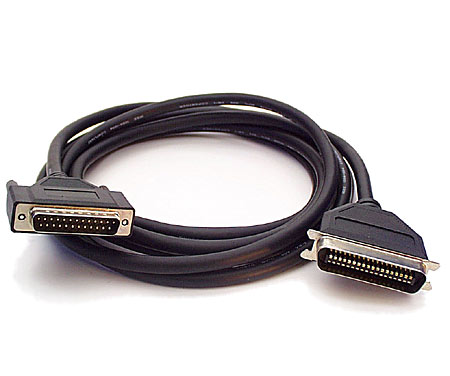
\includegraphics[scale=0.5]{./pics/IEEE1284Printercable_2007_04.jpg}
 \caption{IEEE 1284-Druckerkabel (Typ AB)} 	
\end{figure}
Der IEEE-Standard definiert die elektrischen Eigenschaften der Schnittstellen, die zu verwendenden Hardwareprotokolle und die zugehörigen Kabel. Für softwareseitige Protokolle wird auf Substandards verwiesen, die u.a. auch unabhängig von der eigentlichen Hardware agieren können. Heutzutage ist die parallele Schnittstelle (LPT) größtenteils durch modernere Schnittstellen, wie USB, ersetzt worden und erfährt nicht mehr die gleiche Bedeutung wie noch in den 1990er Jahren. 

 
\subsection{Aufgabenstellung und Projektziel}

Moderne PCs und Notebooks verzichten heutzutage bereits oft auf die parallele Schnittstelle und bieten für zusätzliche Peripheriegeräte dafür USB-Anschlüsse. Zwar sieht der ATX-Gehäusestandard noch farbliche Kennungen für LPT-Schnittstellen vor, bindend muss aber kein Hersteller diese Schnittstelle auf seinen Platinen integrieren. Um dennoch z.B. ältere Drucker in modernen Systemen verwenden zu können, bietet sich der Einsatz von PCI-Adapterkarten an, die über den PCI-Bus nach Außen hin einen Anschluss für die parallele Schnittstelle liefern. Die Implementierung eines Linux-Treibers einer solchen PCI-Adapterkarte soll Gegenstand dieser Projektarbeit sein. 

\subsection{Eingesetzte Hardware}  

Als Hardwareziel kommt eine PCI-Karte der Firma Exsys Inc (http://www.exsys.com) zum Einsatz, auf der ein Chip der Firma Moschip (http://www.moschip.com/) zum Einsatz kommt. Der dort verwendete Mikrocontroller stellt einen MCS9815-Chip dar, der die PCI zu LPT-Kommunikation übernimmt. Zwar findet sich im Linux-Kernel bereits ein Treiber für diesen Mikrokontroller, aufgrund geringer Projekteressourcen fehlt es jedoch an weiteren Alternativen. Da diese Projektarbeit eher dem lehrhaften Charakter einer studentischen Arbeit entspricht und die PCI-Karte den Projektteilnehmern bereits vorliegt, stellt die Entwicklung eines zusätzlichen Treibers für diese Karte nicht nur eine gute Übung dar, sondern ist auch gleichzeitig eine Herausforderung eine tatsächlich existierende Hardware unter dem Betriebssystem Linux zum Laufen zu bringen. Die Spezifikation dieses Mikrokontrollers hat die Firma Moschip offen gelegt, wodurch die Implementierung eines Treibers im Rahmen einer Projektarbeit ermöglicht wird.    


\section{Parallelportschnittstelle}

Die Parallelportschnittstelle ist wesentlich durch den IEEE 1284-Standard geprägt und definiert drei mögliche Steckertypen. Auf PC-Seite findet sich ein 25-poliger D-SUB.Stecker, der 1981 von IBM im PC eingeführt wurde (\textbf{Typ A}). Die 36-polige Centronics-Schnittstelle stellt den Stecker vom \textbf{Typ B} dar. Als Mini-Centronics werden Stecker vom \textbf{Typ C} bezeichnet, die ebenfalls über 36 Pole verfügen, aber deutlich kompakter daherkommen als übliche Centronics-Stecker. 

\begin{figure}[h!]
 \centering
 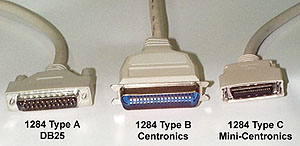
\includegraphics{./pics/ieee1284_types.jpg}
 \caption{Alle IEEE 1284-Steckertypen im Vergleich} 	
\end{figure}


Üblicherweise wurden bei der häufig vorkommenden Verbindung zwischen PC und Drucker Kabel vom Typ AB eingesetzt. Dabei muss ein Mapping vom 25-poligen Typ A-Anschluss zum 36-poligen Typ-B-Anschluss vorgenommen werden (siehe Abbildung).  


\begin{figure}[h!]
 \centering
 
\includegraphics[scale=0.7]{./pics/ieee1284_pinbelegungAB.png}
 \caption{Pinbelegung und -Verdrahtung bei üblichen Druckerkabeln} 	
\end{figure} 

 
 Die folgende Tabelle beschreibt die  Belegung und Bedeutung der einzeln Pins bei einem üblichen Druckerkabel. 
 \\ \\
 \begin{tabular}{|p{20mm}|p{20mm}|c|c|c|c|}
  \hline
	Pin (SUB-D-Type 25) & Pin (Centronics) & SPP Signal & Richtung Out & Register & Hardware\\ \hline
	1 & 1	& 	Strobe					& 	Out		&	Control	&	Ja	\\ \hline
	2 & 2	&	Data 0					&	Out		& 	Data		&     \\ \hline
	3 &	3	&	Data 1				&	Out		&	Data		&     \\ \hline
	4 &	4	&	Data 2				&	Out		&	Data		&     \\ \hline
	5 &	5	&	Data 3				&	Out		&	Data		&     \\ \hline
	6 &	6	&	Data 4				&	Out		&	Data		&     \\ \hline
	7 &	7	&	Data 5				&	Out		&	Data		&     \\ \hline
	8 &	8	&	Data 6				&	Out		&	Data		&     \\ \hline
	9 &	9	&	Data 7				&	Out		&	Data		&     \\ \hline
	10 & 10	&	Ack					&	In		&	Status	&	    \\ \hline
	11 & 11	&	Busy					&	In		&	Status	&	Ja  \\ \hline
	12 & 12	&	Paper-Out/Paper-End	&	In		&	Status	&	    \\ \hline
	13 & 13	&	Select				&	In		&	Status	&	    \\ \hline
	14 & 14	&	Auto-Linefeed			&	Out		&	Control	&	Ja  \\ \hline
	15 & 32	&	Error					&	In		&	Status	&	    \\ \hline
	16 & 31	&	Reset				&	Out		&	Control	&	    \\ \hline
	17 & 36	&	Select-Printer/Select-In	&	Out		&	Control	&	Ja  \\ \hline
	18 - 25	&	19-30				&	Ground	&	Gnd	&	&             \\ \hline
 \end{tabular}


%Um die einzelnen Pins mit Signalen zu belegen, sind drei Speicherbereiche (Ports) für die Behandlung der LPT-Schnittstelle im Rechner vorgesehen.  \\\\
% \begin{tabular}{|c|c|c|c|}
% \hline
%\multicolumn{3}{|l|}{Portadresse}	&	Funktion\\  \hline 
%278	&	378	&	3BC	&	Datenport \\  \hline 
%279	&	379	&	3BD	&	Statusport \\  \hline 
%27A	&	37A	&	3BE	&	Steuerport \\  \hline 
% \end{tabular} 
 
In der Regel werden die Bereiche 278-27A und 378-37A verwendet. Der \textbf{Datenport} ist ein 8-Bit-Ausgagsport, der den Datenleitungen der parallelen Schnittstelle entspricht.  Der \textbf{Steuerport} setzt sich aus  Strobe, Auto-Feed, Reset, Select printer, IRC7 enable und Direction zusammen. 
 \begin{tabular}{|c|c|c|c|}
  \hline
Bit	&	Funktion		&	Pegel  \\ \hline
0	&	Strobe		&	0 \\ \hline
1	&	Auto-Feed		&	1\\ \hline
2	&	Reset		&	0\\ \hline
3	&	Select printer	&	1\\ \hline
4	&	IRQ7 enable	&	1\\ \hline
5	&	Direction	&	1\\ \hline
 \end{tabular} 

\section{Der MosChip MCS9815 Controller}

Der MCS9815 ist ein Parallelport Controller Chip der Firma MosChip. Er kann
zwei Parallelports über das PCI Interface an das System anbinden und unterstützt alle
aktuellen Modi (SPP, PS2, EPP, ECP) der Parallelschnittstelle (vgl. Abbildung \ref{fig:blockdiagramm_mcs9815}).

\begin{figure}[h!]
 \centering
 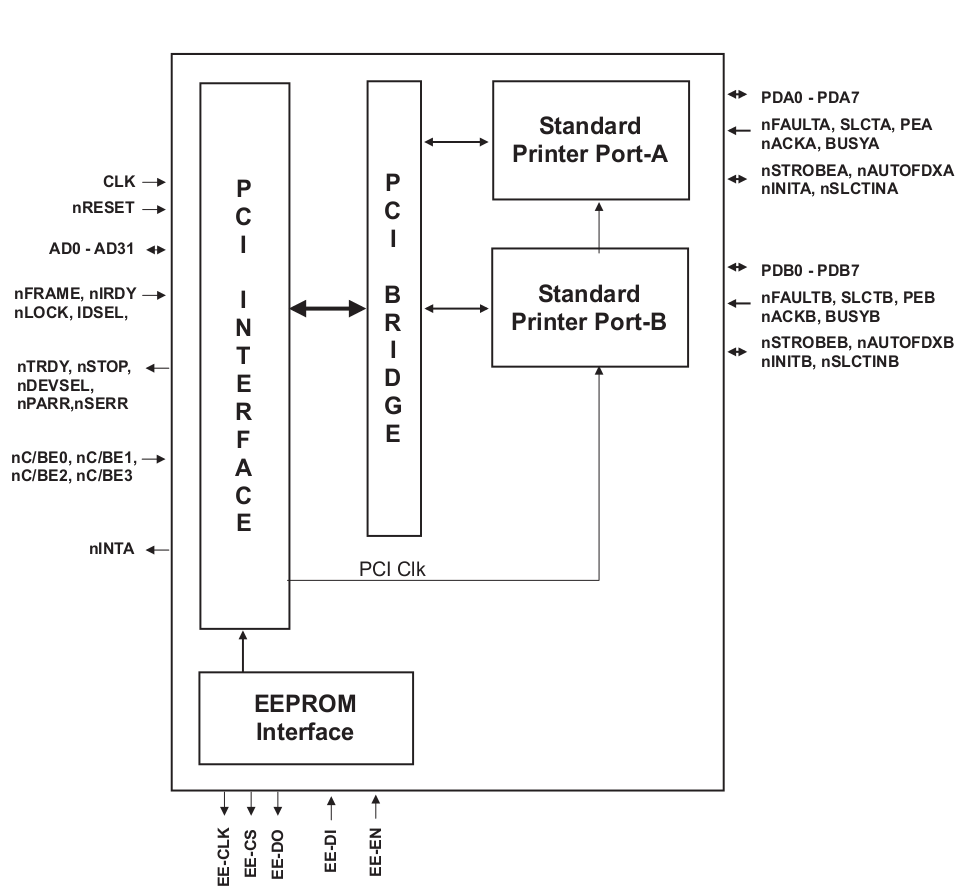
\includegraphics[bb=0 0 724 671,scale=0.5]{./pics/mcs9815_block_diagram.png}
 \caption{Blockdiagramm des MosChip MCS9815}
 \label{fig:blockdiagramm_mcs9815}
\end{figure}

Einschränkungen des Chips ist die fehlende RLE-Kompression der Daten im ECP-Modus. Da dieser Modus aber
in der Praxis selten verwendet wird, ist diese Einschränkungen zu vernachlässigen.
Auch DMA (Direct-Memory-Access) unterstützt der Baustein nicht. Diese Informationen lassen sich dem Config-B Registers des
Chips entnehmen (oder auch dem Spezifikationsdokument des Chips \cite{net:3}).
Die aufwändige Handshaking beim EPP-Modus kann die der MCS9815 in der Hardware abhandeln.

\section{Parport-Treiber in Linux}

\subsection{Aufbau des parport-Subsystems}

Da die Parallelportschnittstelle aus der Steinzeit der PC-Entwicklung stammt, ist die Unterstützung
dafür im Linux-Kernel sehr gut. 
Das \verb|parport| Subsystem besteht im Wesentlichen aus zwei Teilbereichen, einem abstrakteren Highlevel-System, das
die IEEE 1284 Kommunikation beherrscht und einem Lowlevel-System, was den Hardwarezugriff auf die einzelnen Ports
kontrolliert. Auf einem PC stellt das Modul \verb|parport_pc| den architekturspezifischen Teil bereit, das Modul \verb|parport| 
den generischen Teil (vgl. \cite{net:1} und Abbildung \ref{fig:parport_struktur}).

\begin{figure}[h!]
 \centering
 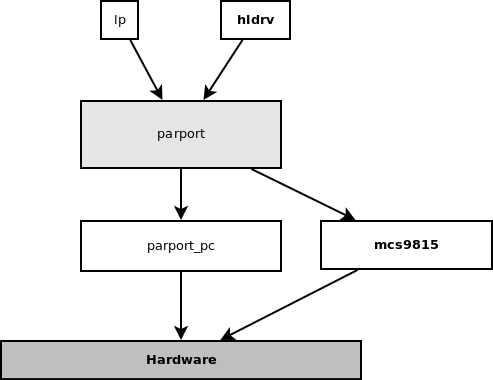
\includegraphics[scale=0.7,bb=0 0 493 380]{./pics/parport_struktur.png}
 \caption{Das parport-Modul stellt eine abstrakte Schnittstelle für Gerätetreiber bereit, die Brücke zur Hardware schlagen Architektur- und Hardware-
spezifische Treibermodule}
\label{fig:parport_struktur}
\end{figure}

Der hardwarespezifische Treiber registriert einen \emph{Port}\footnote{Port ist hier die logische Parallelschnittstelle, nicht zu verwechseln
mit dem I/O-Port (z.B. 0x378), der im PC für den Zugriff auf die Parallelporthardware verwendet werden kann} 
im \verb|parport| Subsystem. 
Dieses benachrichtigt alle registrierten Highlevel-Treiber (z.B. der Gerätetreiber \verb|lp| für Drucker) über den neuen Port. Der Lowlevel-Treiber stellt
Funktionen für den Zugriff auf Basisfunktionen des Ports bereit (vgl. \cite{net:1}).

Aufgabe dieser Hausarbeit ist es, einen Lowlevel-Treiber für einen speziellen Parallelport-Controller zu schreiben. Diese 
Funktionalität ist normalerweise im architekturspezifischen Modul \verb|parport_pc| integriert.

\subsection{Aufbau des MCS9815-Treibers}

In der Struktur des Treibersystems ordnet sich der im Rahmen dieser Arbeit zu erstellende Treiber als hardwarespezifischer Treiber
zwischen dem generischen parport-Modul und der eigentlichen Hardware ein. Er ist also der Adapter zwischen Hardware und parport-Modul 
(vgl. Abbildung \ref{parport_struktur}).

Die verwendete Schnittstellenkarte Exsys EX-41012 wird über den PCI-Bus an das System angebunden. Aufgabe des Treibers nach der generellen
Modulinitialisierung ist die Registrierung des Moduls als PCI-Treiber. Dies geschieht über den Aufruf der Kernelfunktion
\verb|pci_register_driver| mit einer entsprechenden \verb|pci_driver|-Struktur.

Sobald der Kernel die PCI-Karte mit der entsprechenden PCI-ID detektiert, wird die \verb|pci_probe| Funktion des Treibers aufgerufen, die
daraufhin mit der Initialisierung diverser Strukturen für das parport-Subsystem beginnt. Diese Aufgabe übernimmt die Funktion \verb|init_parport|
in der Datei\verb| mcs9815_main.c|.
Sie fragt den Kernel u.a. nach den I/O-Ports, über die die Kommunikation mit der Hardware abläuft. Der MCS9815-Controllerchip verwendet pro
Parallelport zwei Base-Address-Register (BAR). Wie die Parallelportregister auf die BARs der PCI-Hardware gemappt sind, zeigt 
Abbildung \ref{portkonf_mcs9815}.

\begin{figure}[h!]
 \centering
 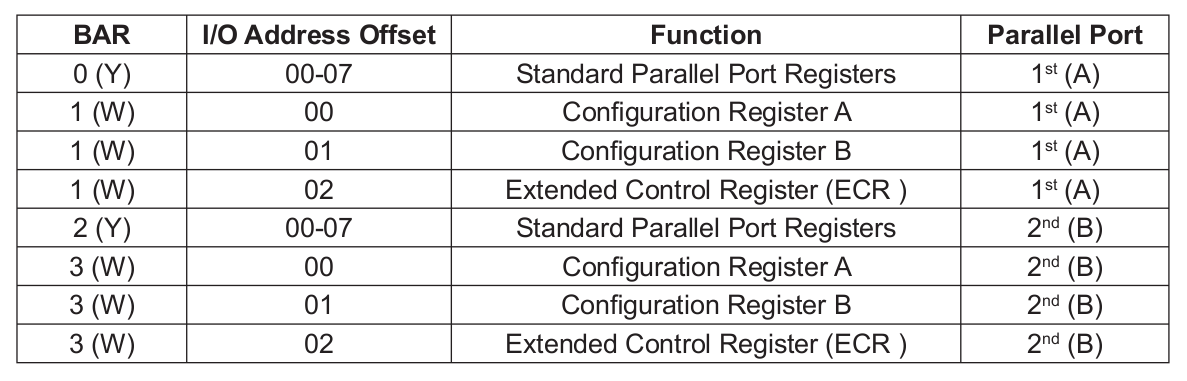
\includegraphics[scale=0.5]{./pics/mcs9815_ioports.png}
 \caption{Portkonfiguration des MosChip MCS9815}
 \label{portkonf_mcs9815}
\end{figure}

Sobald die entsprechenden I/O-Ports bestimmt wurden, werden sie vom Treiber mit der Kernelfunktion \verb|request_region| allokiert.
Des weiteren füllt die \verb|init_parport| Funktion die Instanz der \verb|parport| Struktur mit sinnvollen Werten.
Die Struktur \verb|parport| repräsentiert eine logische Parallelschnittstelle.

\begin{verbatim}
struct parport {
    struct parport *next; /* next parport in list */
    const char *name;     /* port's name */
    unsigned int modes;   /* bitfield of hardware modes */
    struct parport_device_info probe_info;
                          /* IEEE1284 info */
    int number;           /* parport index */
    struct parport_operations *ops;
};\end{verbatim}

Die Struktur enthält auch einen Verweis auf die wichtige Struktur \verb|parport_operations|.
Wie auch die Struktur \verb|file_operations| bei einem Dateisystemtreiber enthält die 
Struktur \verb|parport_operations| u.a. Funktionszeiger auf die vom Treiber unterstützten
Parallelportfunktionen.

\begin{verbatim}
struct parport_operations {
    /* IBM PC-style virtual registers. */
    void (*write_data)(struct parport *, unsigned char);
    unsigned char (*read_data)(struct parport *);

    void (*write_control)(struct parport *, unsigned char);
    unsigned char (*read_control)(struct parport *);
    unsigned char (*frob_control)(struct parport *, unsigned char mask, unsigned char val);

    unsigned char (*read_status)(struct parport *);

    /* IRQs. */
    void (*enable_irq)(struct parport *);
    void (*disable_irq)(struct parport *);

    /* Data direction. */
    void (*data_forward) (struct parport *);
    void (*data_reverse) (struct parport *);

    /* For core parport code. */
    void (*init_state)(struct pardevice *, struct parport_state *);
    void (*save_state)(struct parport *, struct parport_state *);
    void (*restore_state)(struct parport *, struct parport_state *);

    /* [..] */

    size_t (*compat_write_data) (struct parport *port, const void *buf, size_t len, int flags);
    size_t (*nibble_read_data) (struct parport *port, void *buf, size_t len, int flags);
    size_t (*byte_read_data) (struct parport *port, void *buf, size_t len, int flags);
    struct module *owner;
};\end{verbatim}

Das generische parport Modul des Kernels verwendet diese Funktionszeiger um über das hardwarespezifische Modul mit 
der tatsächlichen Hardware zu kommunizieren.
Die Implementierung dieser Funktionen befinden sich in der Datei \verb|mcs9815_ops.c|. 

Mit den entsprechend initialisierten Strukturen registriert der Treiber mit dem Aufruf der Funktion \verb|parport_register_port| einen Parallelport im Kernel.
Um diesen Parallelport den Gerätetreibern im System bekannt zu machen, muss die Funktion \verb|parport_announce_port| aufgerufen werden.
Wie ein (highlevel) Gerätetreiber das parport-Subsystem verwendet wird im folgenden Abschnitt erläutert.
Nach dem Bekanntmachen des Treibers ist die Initialisierung abgeschlossen und der Treiber kann verwendet werden.
Beim Entfernen des Treibers aus dem System wird der Parallelport vom Kernel abgemeldet, die Strukturen abgemeldet und schließlich das PCI-Gerät 
abgeschaltet.

\subsection{Highlevel Testtreiber}

\section{Fazit}

Zum Status des Treibers ist zu sagen, dass er
nur im SPP-Modus getestet wurde. Die EPP-Funktionen sind zwar vollständig implementiert, aber mangels Testgerät ungetestet.
Die ECP-Funktionen konnten aus Zeitgründen nicht mehr vollständig implementiert und getestet werden.

\bibliography{literatur}


\end{document}